\documentclass{optica-article}

\journal{opticajournal} % for journals or Optica Open

\articletype{Research Article}
\usepackage{float}
\usepackage{lineno}
\linenumbers % Turn off line numbering for Optica Open preprint submissions.

\usepackage{fancyhdr}

\pagestyle{fancy}
\fancyhf{}
\rfoot{\thepage}

\begin{document}

\title{Generating Random Surfaces for Thermal Emission Studies}



\author{Abhishek,\authormark{1,*}, Guneshwar Thangjam,\authormark{1,+}}

\address{\authormark{1}National Institute of Science Education and Research, Jatni, Khordha 752050, Odisha, India}

\email{\authormark{*}abhishek.2019@niser.ac.in} %
\email{\authormark{+}thangjam@niser.ac.in}


\begin{abstract*}
	This report presents different methods to generate random surfaces for 
	thermal emission studies. The methods include the generation of random surfaces of several shapes
	and sizes using the Python programming language. Most of the methods are employed from the two sources~\cite{WOHLER2017118}
	and~\cite{DAVIDSSON20151}. My part of the work is to implement the methods in Python and 
	generate the random surfaces. In addition, the report also presents the solution of the 1D heat equation for the moon's surface.
	
\end{abstract*}

%%%%%%%%%%%%%%%%%%%%%%%%%%  body  %%%%%%%%%%%%%%%%%%%%%%%%%%
\section{Introduction}

The Moon Mineralogy Mapper ( $M^{3}$)~\cite{chandrayaan1} radiance spectra on the lunar surface include a thermal emission component 
that becomes significant around 2.2 $\mu$m, particularly in the 2.8–3.0 $\mu$m 
range where water and hydroxyl (OH) absorption features are present. 
To interpret these spectra, compensation for the local surface temperature is 
required.

Clark et al. (2011)~\cite{clark_thermal_2011} proposed a complex method for temperature estimation that 
involves comparing different parts of the reflectance spectrum. However, 
this method can be imprecise, particularly in regions with strong pyroxene 
absorptions, and it often fails to fully account for thermal emissions in the 
OH absorption range.

Wöhler et al. (2014)~\cite{WOHLER201486} suggested a simpler method, which combines a standard 
lunar sample spectrum and a blackbody spectrum. However, their estimates are 
often too low for surface temperatures below 250–280 K.

Li and Milliken (2016)~\cite{li_empirical_2016} introduced another approach using a thermal emission 
model and a reflectance model to estimate temperature. While this method is 
more accurate, it still has difficulties in areas rich in certain minerals 
and at high incidence angles.

In response to these issues, the researchers developed two new methods. 
One method calculates solar energy per surface element and models thermal energy 
flow within lunar soil. The other method derives surface properties 
from M³ measurements.

\section{Effects of Surface Roughness on Thermal Emission}

A smooth surface emits radiation uniformly in all directions, and its temperature 
corresponds to the observed brightness temperature. However, a rough surface, 
with its uneven angles and shadows, 
exhibits significant temperature variations across its extent. Consequently,
 the observed radiation is not uniformly distributed and does not correspond to 
 a single temperature. Instead, it depends on the incidence of sunlight and the 
 viewing geometry. If sunlight predominantly strikes directly and we observe those
  regions, the observed radiation is higher, a phenomenon known as beaming. 
  Conversely, if there are many shadows, the observed radiation is lower. 
  Surface roughness significantly influences the emitted radiation.

Under normal circumstances, we can estimate the surface temperature from the 
emitted radiation using Planck's law:

\begin{equation}
B(\lambda,T) = \frac{2hc^2}{\lambda^5} \frac{1}{e^{\frac{hc}{\lambda kT}} - 1}
\end{equation}

where $B(\lambda,T)$ is the spectral radiance at wavelength $\lambda$ and 
temperature $T$.
However, the emission spectra of rough surfaces comprise several components 
emitting a superposition of several wavelengths due to heat diffusion and 
self-heating of the surface. As a result, it is not possible to accurately 
determine the temperature using Planck's law.


\section{Different Topographies of the Moon's Surface}

%%concave spherical segments
\subsection{Concave Spherical Segments}\label{sec:concave}

 A 1 $m^2$ area in the $x-y$-plane is divided into a quadratic grid with 
1024 squares. Each node on the grid is assigned a $z$-value, 
which is zero outside a circular rim centered on $x = y = 0$ with 
radius $r = 0.437$ m, to produce a crater coverage of $f = 0.6$. 
Within the rim, the $z$-coordinate is given by 

\begin{equation}
z = R - h - \sqrt{R^2 - x^2 - y^2}
\end{equation}

This gives the terrain within the rim the shape of a concave spherical 
segment. Here, $h$ is the crater depth and $R = \frac{r^2 + h^2}{2h}$ is 
the curvature radius of the spherical segment. By varying $h$, we obtain 
different degrees of roughness.
The four nodes on the terrain surface corresponding to a particular square 
in the $xy$-plane are used to form two triangular facets. The total number
 of triangular facets on the surface is thus 2048. For each facet, 
 we calculate the surface area, the normal vector, and its tilt with respect to the $z$-axis.
 These are used to calculate the RMS slope angle $s$ according to Eq. (1).
There are several types of spherical segment terrains with $s = 5^\circ$, $20^\circ$, and 
$35^\circ$ by using $h = 0.0359$ m, $0.151$ m, and $0.313$ m, respectively. In this study,
only the $s = 35^\circ$ terrain is considered and reconstructed.

\begin{figure}[ht]
    \centering
	\hspace{-1cm}
    \begin{minipage}{0.45\textwidth}
        \centering
        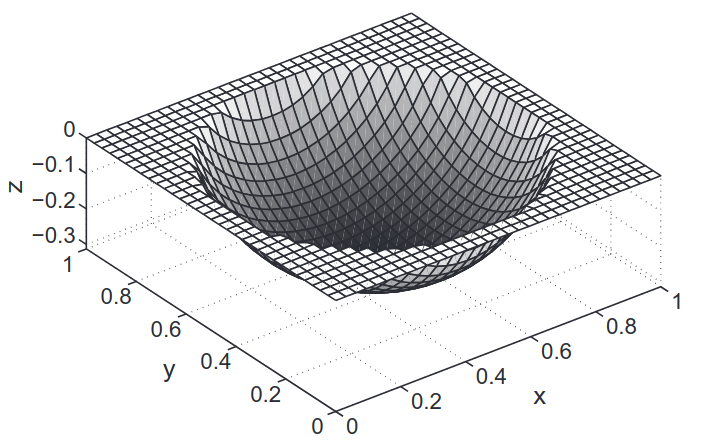
\includegraphics[width=\textwidth, height = 4cm]{./Figures/concave_d.png} 
        \caption{Concave spherical segment with $s=35^\circ$~\cite{DAVIDSSON20151}.}
        \label{fig:concave_d}
    \end{minipage}\hfill
	\hspace{-0.8cm}
    \begin{minipage}{0.45\textwidth}
        \centering
        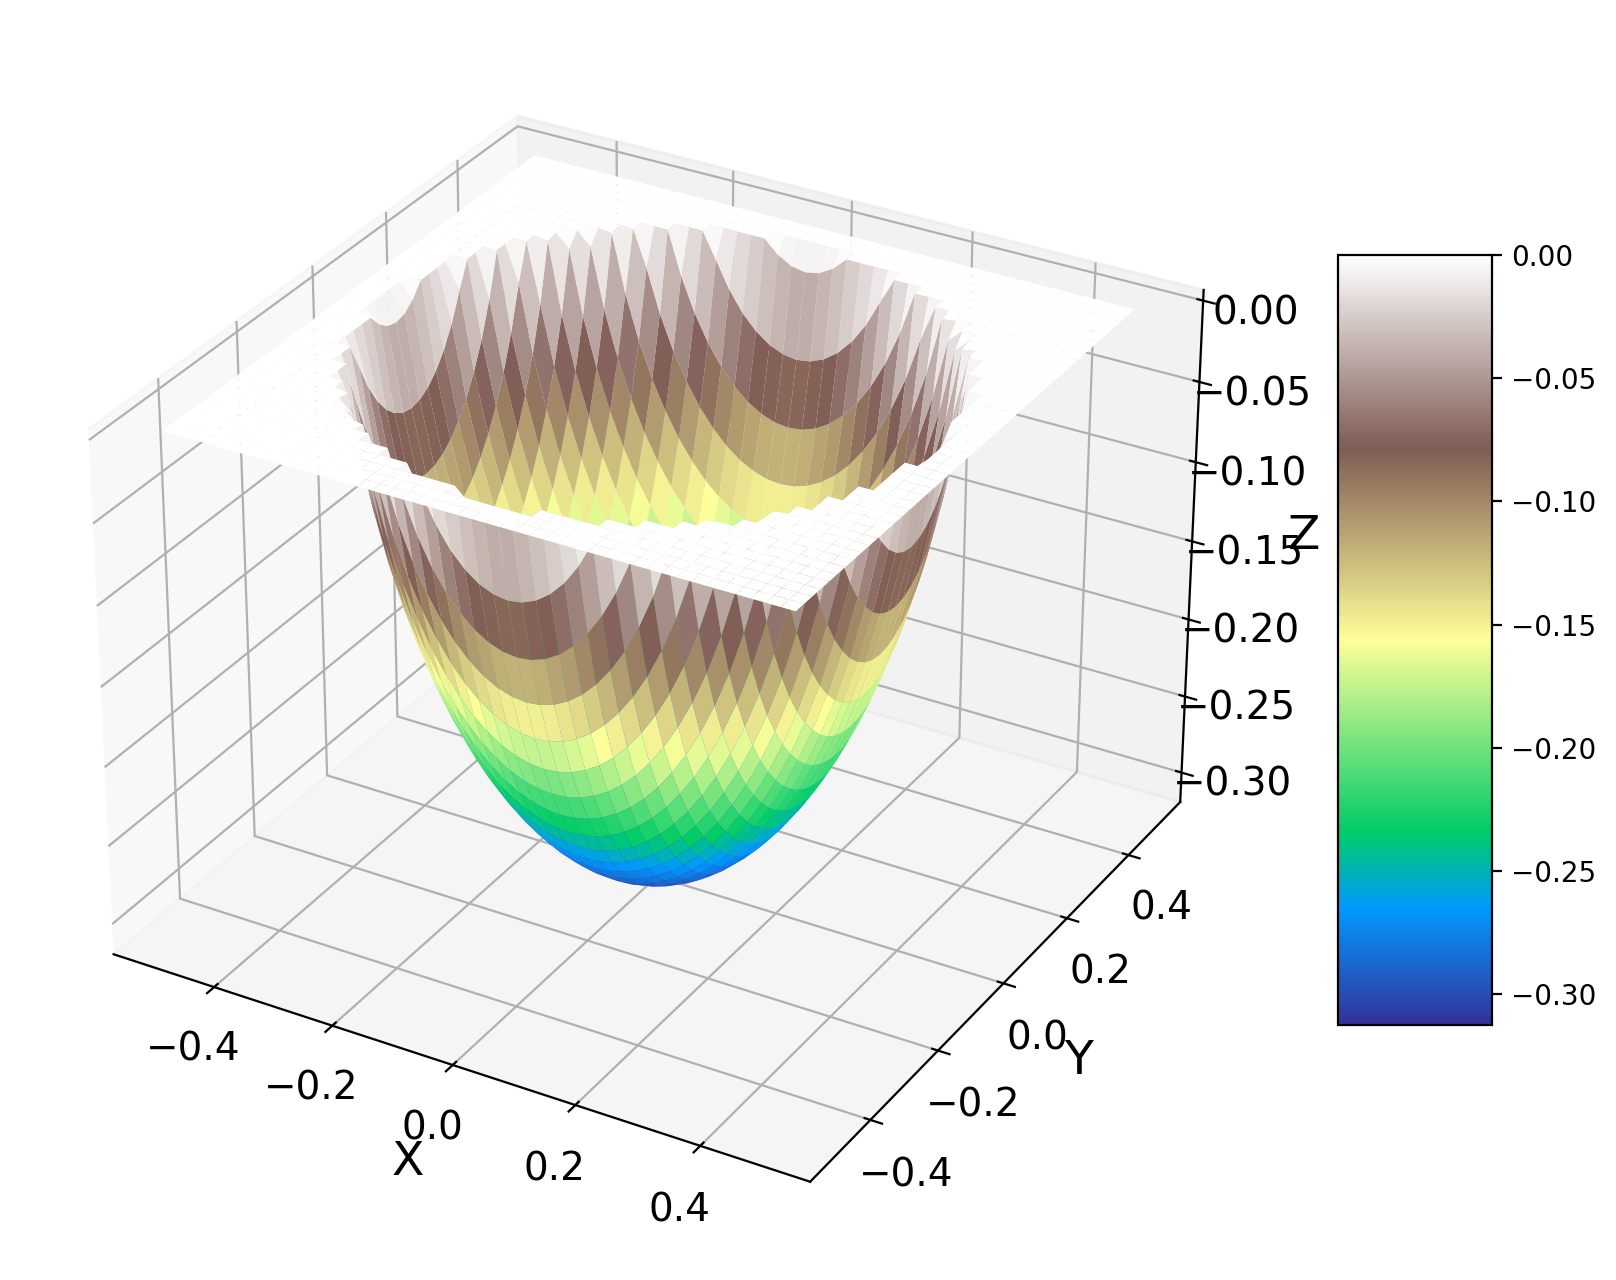
\includegraphics[width=\textwidth]{./Figures/concave.png} 
        \caption{Reconstructed concave spherical segment with $s = 35^\circ$.}
        \label{fig:concave}
    \end{minipage}
\end{figure}

In Figure~\ref{fig:concave_d}, a topography of concave spherical segment with $s = 35^\circ$ is shown which is 
takem from~\cite{DAVIDSSON20151}. The reconstructed concave spherical 
segment with $s = 35^\circ$ is shown in Figure~\ref{fig:concave}.

%%%parallel sinusoidal trenches
\subsection{Parallel sinusoidal trenches}
To create parallel sinusoidal trenches, we use the same quadratic grid as in Section~\ref{sec:concave},
 but with z-coordinates determined by $z = C_t + C_t \sin(2\pi(N_{\text{trench}} + 0.5)x)$, 
 resulting in three trenches parallel to the y-axis. The amplitude $C_t$ controls the roughness level. 
We construct 2048 triangular surface facets based on Cartesian node positions and calculate $s$ as for 
spherical segments. To achieve $s = 5^\circ$, $20^\circ$, and $35^\circ$, we set $C_t = 0.00575$ m, $0.02438$ m, and $0.04912$ m, respectively. 
In this study, only the $s = 35^\circ$ terrain is considered and reconstructed.

\begin{figure}[H]
    \centering
	\hspace{-1cm}
    \begin{minipage}{0.45\textwidth}
        \centering
        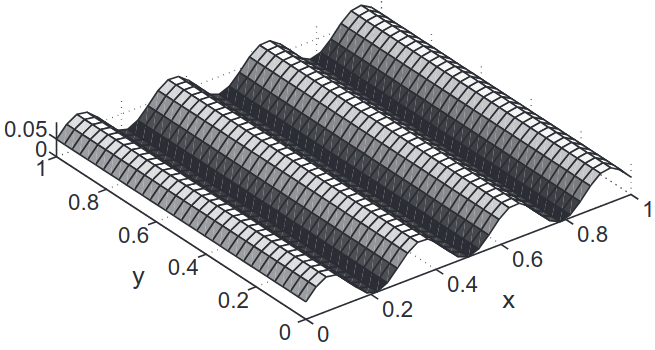
\includegraphics[width=\textwidth, height = 4cm]{./Figures/sin_d.png} 
        \caption{sinusoidal trenches with $s=35^\circ$~\cite{DAVIDSSON20151}.}
        \label{fig:sin_d}
    \end{minipage}\hfill
	\hspace{-0.8cm}
    \begin{minipage}{0.45\textwidth}
        \centering
        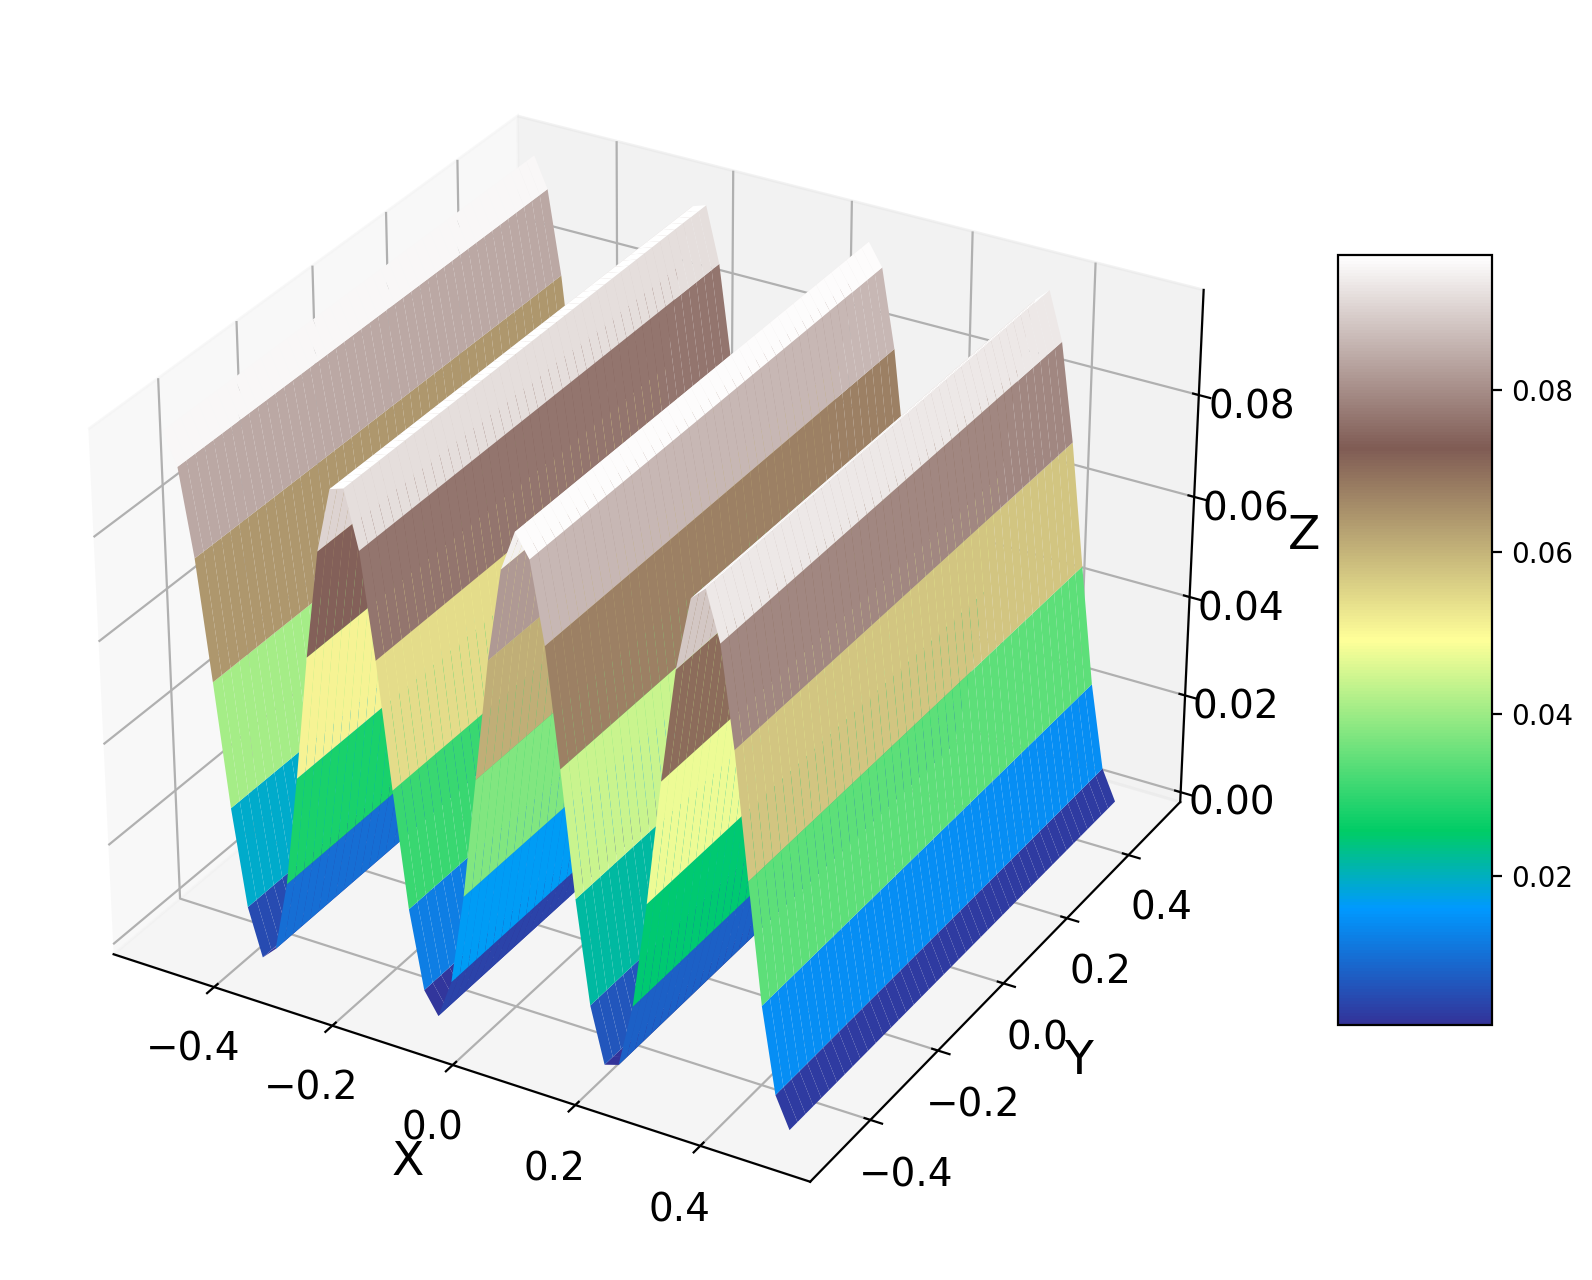
\includegraphics[width=\textwidth]{./Figures/sin.png} 
        \caption{Reconstructed sinusoidal trenches  with $s = 35^\circ$.}
        \label{fig:sin}
    \end{minipage}
\end{figure}

In Figure~\ref{fig:sin_d}, a topography of sinusoidal trenches with $s = 35^\circ$ is 
shown which is reconstructed as shown in Figure~\ref{fig:sin}.

%%%Random Gaussians
\subsection{Random Gaussians}
Random numbers are required to generate random surfaces. The random numbers are generated 
using the linear congruential generator (LCG) method that was taught in the course. 

\begin{itemize}
	\item The function \texttt{lcg(modulus, a, c, seed)} is defined to implement a Linear Congruential Generator (LCG). The LCG is a type of pseudorandom number generator algorithm that yields a sequence of pseudorandom numbers. The LCG uses the equation $X_{n+1} = (aX_n + c) \mod m$ to generate the next number in the sequence, where:
		\begin{itemize}
		\item $X_n$ is the current number in the sequence (the seed for the first number),
		\item $a$ is the multiplier,
		\item $c$ is the increment,
		\item $m$ is the modulus.
		\end{itemize}
	\item The parameters for the LCG are defined as follows:
		\begin{itemize}
		\item \texttt{modulus = $2^{32}$}: The modulus $m$ is set to $2^{32}$.
		\item \texttt{a = 1103515245}: The multiplier $a$ is set to 1103515245.
		\item \texttt{c = 12345}: The increment $c$ is set to 12345.
		\item \texttt{seed = int.from\_bytes(os.urandom(4), byteorder="big")}: Sets the seed $X_0$ to a random 32-bit integer from the OS's random number source.
		\end{itemize}
	\item The function \texttt{lcg} is a generator function that, when called, returns an iterator that yields pseudorandom numbers in the range $[0, 1)$.
	\end{itemize}

\subsubsection{2D random Gaussian surface using correlation length}
This method is employed from the source~\cite{mrnka2017random}.
A random surface is defined by the function $h = f(x, y)$, where $h$ denotes the 
height at a given position $(x, y)$. This height, represented by the variable $h$, 
is subject to randomness with a specific mean and standard deviation. 
The characteristics of the surface are determined by two key parameters: 
the root mean square (rms) of the height distribution, denoted as $h_{\text{rms}}$ 
(equivalent to the standard deviation of $h$), and the correlation length $c_l$, 
which governs the spatial frequency of surface variations or the roughness of surface is 
defined using this correlation length. In our isotropic surface,
 both the correlation lengths in the $x$ and $y$ directions are equal and 
 denoted as $c_{lx} = c_{ly} = c_l$.

Following are the steps to generate the random Gaussian surface using correlation length:
\begin{itemize}
	\item Generate a random 2D matrix of size $N \times N$ with random numbers.
	\item Perform a 2D Fourier transform of the random matrix.
	\item N can not be chosen arbitrarily, it should satisfy the Nyquist criterion~\cite{nyquist_shannon}.
	\subitem \[
		\frac{N}{rl} < \frac{2}{cl}
		\]  
		Where $N$ is the number of points on the x and y axis individually, and $rl$ is 
		the length of the x and y sides of the square.	cl is the correlation length.
	\item The final marix is obtained by convolving the random matrix with a Gaussian filter.
	\subitem \[
		G = \exp\left(\frac{x^2 + y^2}{\frac{cl^2}{2}}\right)
		\]
		Here cl is the correlation length. x and y are the coordinates of the matrix for 2D matrix.

	\item The final matrix is obtained by convolving the random matrix with the Gaussian filter.
	\subitem
	\begin{align}
		$$\mathbf{H_f}=\frac{2 L}{\sqrt{\pi} \cdot N \cdot c l} \operatorname{FFT}^{-1}\left(\operatorname{FFT}(\mathbf{H}) \cdot \operatorname{FFT}(\mathbf{G})\right)$$
	\end{align}

\end{itemize}



	Here \textbf{H} is the initial 2D N$\times$N matrix, \textbf{G} is the Gaussian filter, and \textbf{$H_f$} is the 
	final matrix.

	\begin{figure}[H]
		\centering
		\hspace{-1cm}
		\begin{minipage}{0.50\textwidth}
			\centering
			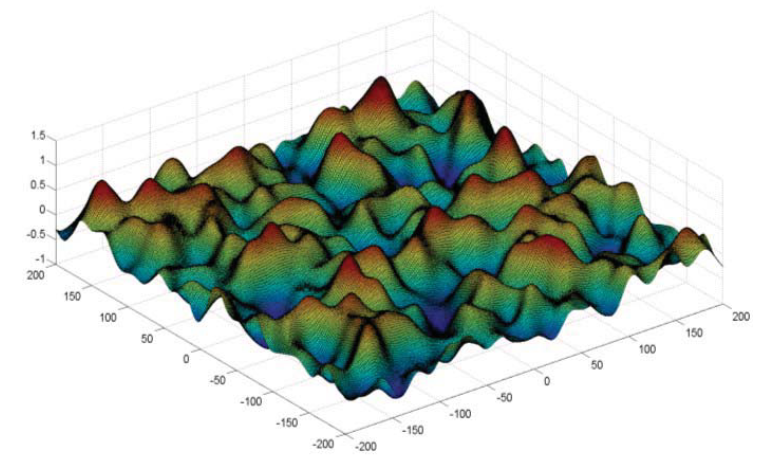
\includegraphics[width=\textwidth]{./Figures/gaussian_i.png} 
			\caption{2D Gaussian random surface taken from the source~\cite{mrnka2017random}.}
			\label{fig:sin_d}
		\end{minipage}\hfill
		\hspace{-0.8cm}
		\begin{minipage}{0.45\textwidth}
			\centering
			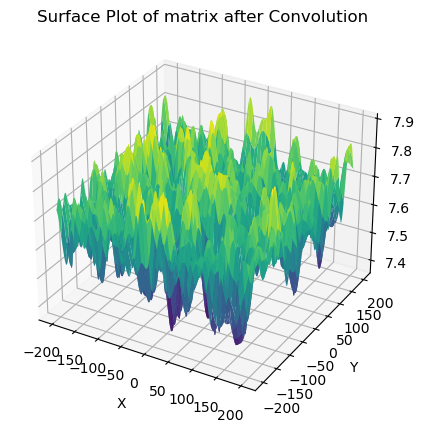
\includegraphics[width=\textwidth]{./Figures/gaussian.png} 
			\caption{Reconstructed 2D Gaussian random surface.}
			\label{fig:sin}
		\end{minipage}
	\end{figure}
			
\subsubsection{2D random Gaussian surface using superposition of multiple Gaussians}
We generate a rough surface using random Gaussians on the same x-y grid as mentioned in Section~\ref{sec:concave}. Each node's z-coordinate is determined by the superimposition of Gaussian functions, which are randomly generated based on amplitude, width, and location.

The z-coordinate of the $(x, y)$ node is given  by following equation:

\[
z(x, y) = z_0(x, y) + A_{\text{gauss}} \exp \left( -\frac{(y - y_0)^2 + (x - x_0)^2}{2\sigma_g^2} \right)
\]

Here, $z_0(x, y)$ is the z-coordinate before the addition of the new Gaussian. The other parameters are defined as:

\[
\begin{aligned}
A_{\text{gauss}} &= C \cdot rn[-1, 1] \\
\sigma_g &= 2.25 + 0.75 \cdot rn[0, 1] \\
x_0 &= 16 \cdot rn[-1, 1] \\
y_0 &= 16 \cdot rn[-1, 1]
\end{aligned}
\]

In these definitions, $rn[-1, 1]$ and $rn[0, 1]$ are real random numbers uniformly generated within the intervals $[-1, 1]$ and $[0, 1]$, 
respectively. $C$ is a constant that varies based on the required roughness level.
 In these simulations, we use $C$ = $0.65$ to create surfaces with 
 $s$ = $35^\circ$.

 \begin{figure}[H]
	\centering
	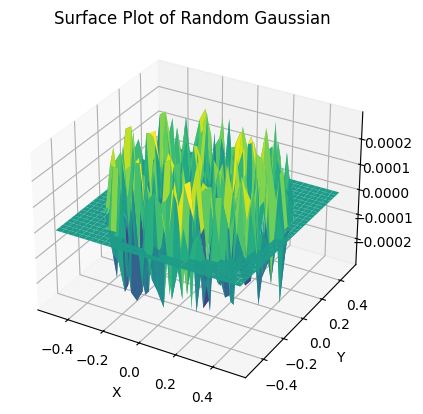
\includegraphics[scale=0.45]{./Figures/gaussian_c.png}
	\caption{2D Gaussian random surface reconstructed using the superposition of multiple gaussians.}
	\label{fig:gaussian_c}	
 \end{figure}


\section{Assumptions and 1D Heat Conduction}

Many researchers have assumed that the size scale of topographic features $D$ is significantly larger than the thermal skin depth $L$ of the surface material. The thermal skin depth is defined as $L = \sqrt{\frac{j}{qcx}}$, where $j$, $q$, and $c$ are the heat conductivity, 
mass density, and specific heat capacity, respectively, 
while $x = \frac{2\pi}{P}$ is the angular velocity, with $P$ being the 
the rotational period of the object under consideration.
The surface temperature fluctuates during rotation, and $L$ is the depth 
under the surface where the amplitude has decreased by a factor 
$e \approx 2.7$ compared to the surface value. Thus, $L$ measures 
the distance over which heat conduction starts to become ineffective in 
transmitting temperature changes from one part of the surface to another.
The assumption that $D >> L$ is used to justify considering only 1D heat 
conduction for the smallest resolution elements of the models. 
Therefore, these researchers neglect lateral heat conduction and the more 
advanced models use a 1D heat equation solver for each facet in the 
plate model that resolves the topographic features.

\subsection{1D Heat Equation using Finite Difference Method}



The finite difference method is a numerical method used for solving 
differential equations. It approximates derivatives by finite differences. 
In the context of the 1D heat equation, which is a parabolic partial 
differential equation, the finite difference method can be used to approximate 
the solution at discrete points in space and time.

\begin{table}[H]
	\centering
	\begin{tabular}{|c|c|}
	\hline
	\textbf{Property} & \textbf{Value} \\
	\hline
	Density & 1800 kg/m$^3$ \\
	\hline
	Heat Capacity & 840 J/(kg.K) \\
	\hline
	Thermal Conductivity & 9.30 $\times$ $10^{-3}$ W/(m.K) \\
	\hline
	\end{tabular}
	\caption{Properties of Moon Regolith~\cite{https://doi.org/10.1029/2021EA001968}}
	\label{tab:moon_regolith_properties}
	\end{table}

	\begin{equation}
		\alpha = \frac{9.3 \times 10^{-3} \times 1800}{ 840} \approx 0.020 \, \text{m}^2/\text{s}
	\end{equation}

The 1D heat equation is given by:

\begin{equation}
\frac{\partial u}{\partial t} = \alpha \frac{\partial^2 u}{\partial x^2}
\end{equation}

where $u$ is the temperature, $t$ is time, $x$ is the spatial coordinate, 
and $\alpha$ is the thermal diffusivity.



To solve this equation using the finite difference method, we discretize 
the spatial domain into $N$ points and the time domain into $M$ points. 
We can then approximate the second derivative in space using the central 
difference scheme and the first derivative in time using the forward difference
 scheme. This leads to the following finite difference equation:

\begin{equation}
\frac{u_i^{n+1} - u_i^n}{\Delta t} = \alpha \frac{u_{i+1}^n - 2u_i^n + u_{i-1}^n}{\Delta x^2}
\end{equation}

where $u_i^n$ is the temperature at spatial point $i$ and time point $n$, 
and $\Delta t$ and $\Delta x$ are the time and space step sizes, respectively.

This equation can be rearranged to give an explicit formula for the temperature 
at the next time step in terms of the temperature at the current and 
neighboring spatial points at the current time step:

\begin{equation}
u_i^{n+1} = u_i^n + \frac{\alpha \Delta t}{\Delta x^2} (u_{i+1}^n - 2u_i^n + u_{i-1}^n)
\end{equation}

This formula can be used to iteratively update the temperature at each point 
in space and time, starting from an initial temperature distribution at 
time $t=0$.

\begin{figure}[H]
	\centering
	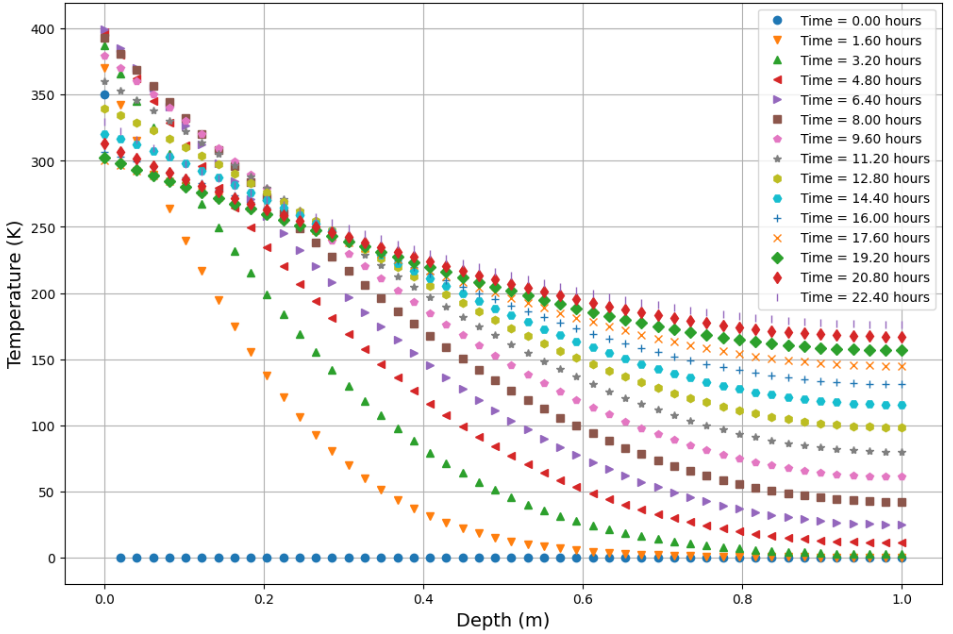
\includegraphics[scale=0.35]{./Figures/heat_eq.png}
	\caption{Solution of the 1D heat equation for the moon's surface.}
	\label{fig:heat_eq}
\end{figure}

Figure~\ref{fig:heat_eq} shows the solution of the 1D heat equation for the moon's surface. 
The temperature distribution is shown at different time steps, illustrating how the temperature 
evolves over time due to heat conduction.

\subsection{Summary}

This report presents the implementation of various methods to generate random surfaces for 
thermal emission studies, particularly focusing on the lunar surface. 
The methods employed are primarily 
derived from two sources~\cite{WOHLER2017118} and~\cite{DAVIDSSON20151}, 
and are implemented using the Python programming language. 

The report discusses different types of topographies 
and the corresponding numerical methods used to generate these surfaces. 
A key component of this work is the development of a random number generator, 
which is utilized to create Gaussian random surfaces. 

In addition to the generation of random surfaces, 
the report also presents the solution of the one-dimensional heat equation for the 
moon's surface. This is achieved through an iterative process over various time steps, 
providing a detailed understanding of the heat conduction within the lunar regolith.




%%%%%%%%%% If using BibTeX:
\bibliography{sample}

%%%%%%%%%% If preparing manually:
% \begin{thebibliography}{1}
% \newcommand{\enquote}[1]{``#1''}

% \bibitem{Zhang:14}
% Y.~Zhang, S.~Qiao, L.~Sun, Q.~W. Shi, W.~Huang, L.~Li, and Z.~Yang,
%   \enquote{Photoinduced active terahertz metamaterials with nanostructured
%   vanadium dioxide film deposited by sol-gel method,}
%   {\protect\JournalTitle{Optics Express}} \textbf{22}, 11070--11078 (2014).

% \bibitem{Optica}
% {Optica}, \enquote{{Optica Publishing Group},}
%   \url{http://www.opg.optica.org}.

% \bibitem{FORSTER2007}
% P.~Forster, V.~Ramaswamy, P.~Artaxo, T.~Bernsten, R.~Betts, D.~Fahey,
%   J.~Haywood, J.~Lean, D.~Lowe, G.~Myhre, J.~Nganga, R.~Prinn, G.~Raga,
%   M.~Schulz, and R.~V. Dorland, \enquote{Changes in atmospheric consituents and
%   in radiative forcing,} in \enquote{Climate Change 2007: The Physical Science
%   Basis. Contribution of Working Group 1 to the Fourth assesment report of
%   Intergovernmental Panel on Climate Change,}  S.~Solomon, D.~Qin, M.~Manning,
%   Z.~Chen, M.~Marquis, K.~B. Averyt, M.~Tignor, and H.~L. Miler, eds.
%   (Cambridge University Press, 2007).

% \end{thebibliography}

\end{document}